\begin{figure*}[!t]
\centering
\subfloat[][Model size]{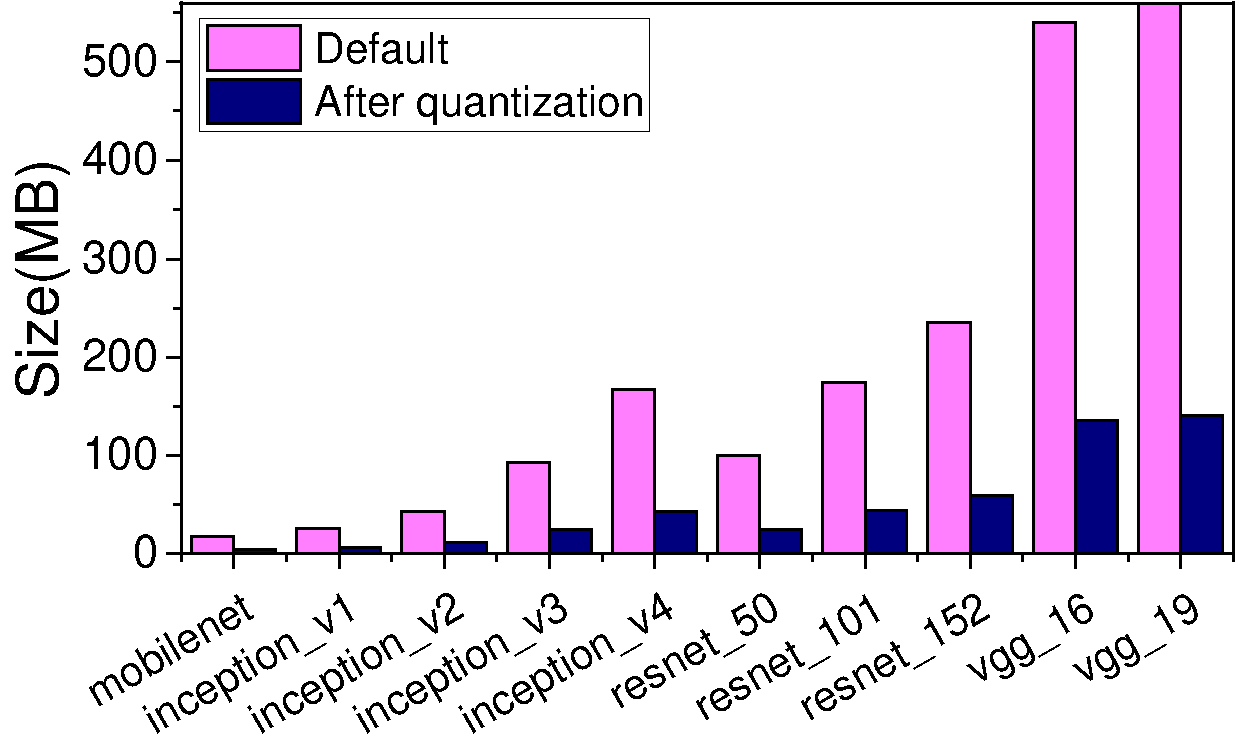
\includegraphics[width=0.33\textwidth]{figure/quan_size.pdf}}
\hfill
\subfloat[][Inference time]{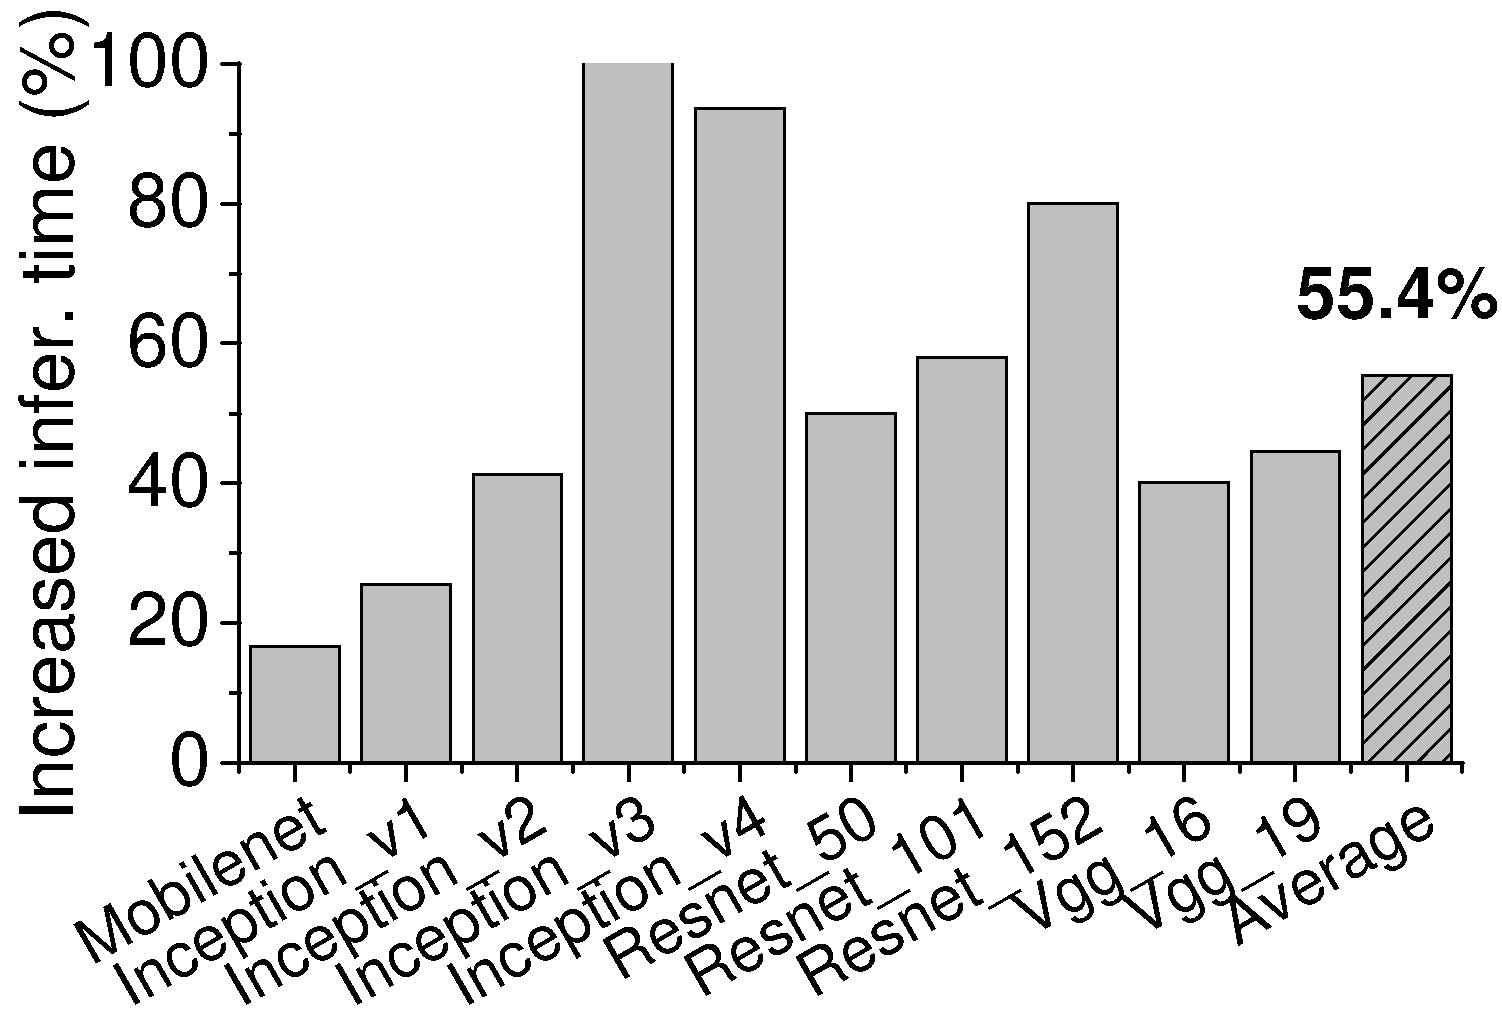
\includegraphics[width=0.3\textwidth]{figure/quan_time.pdf}}
\hfill
\subfloat[][Accuracy]{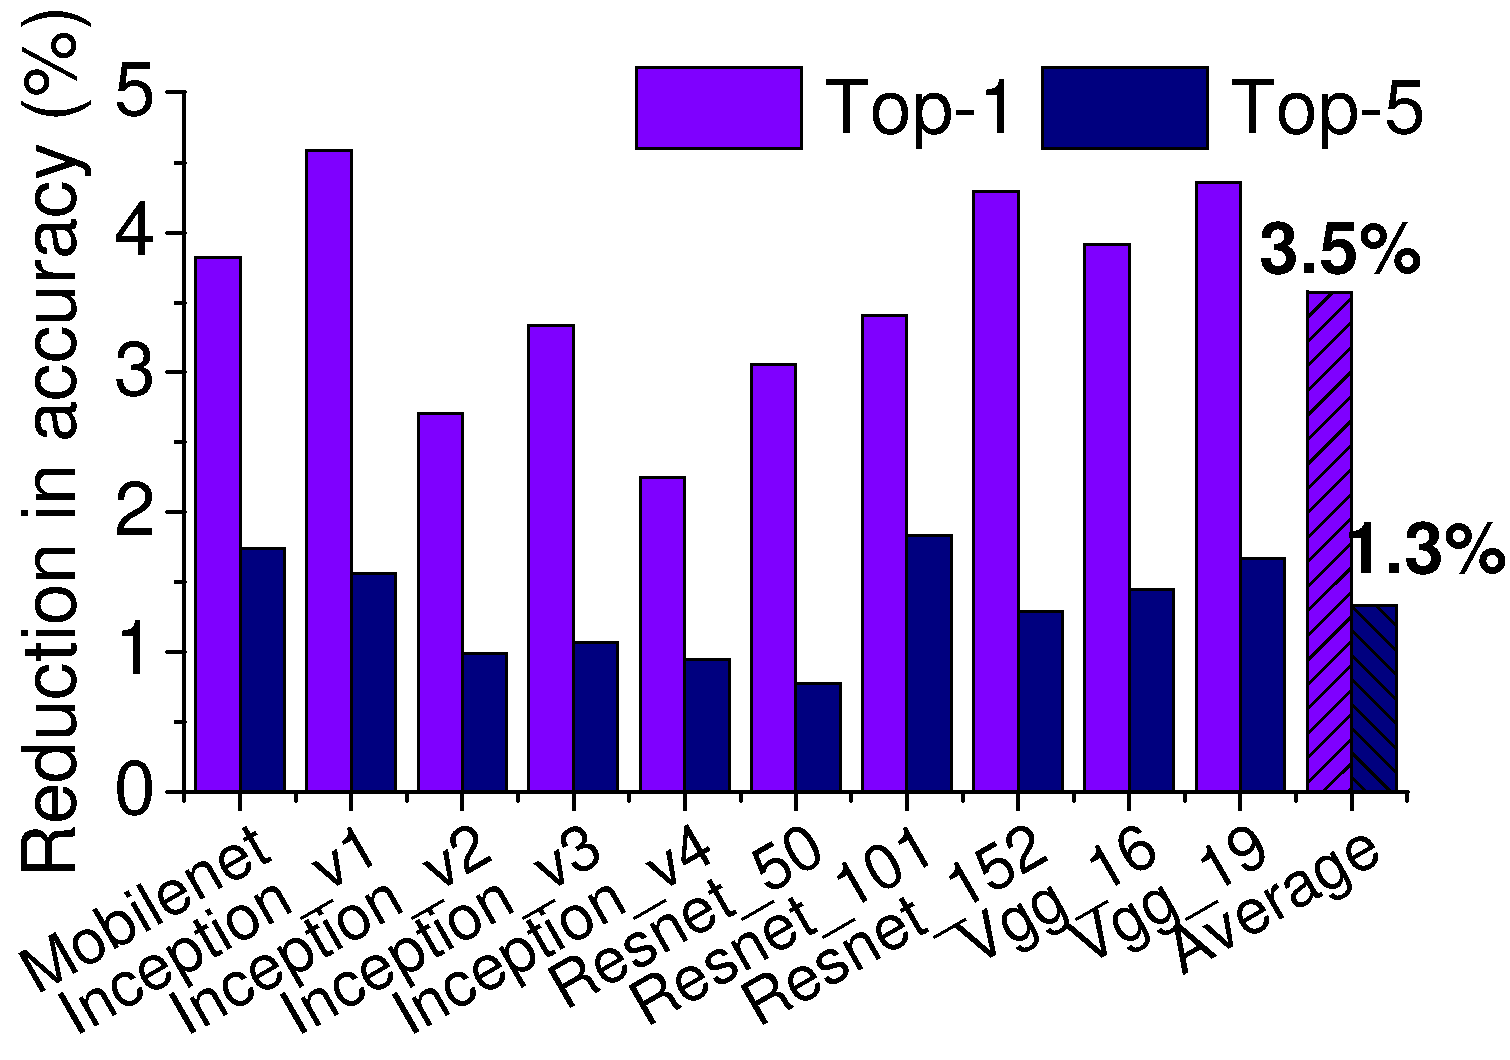
\includegraphics[width=0.3\textwidth]{figure/top1_5_quan.pdf}}
\hfill
\subfloat[][Power consumption]{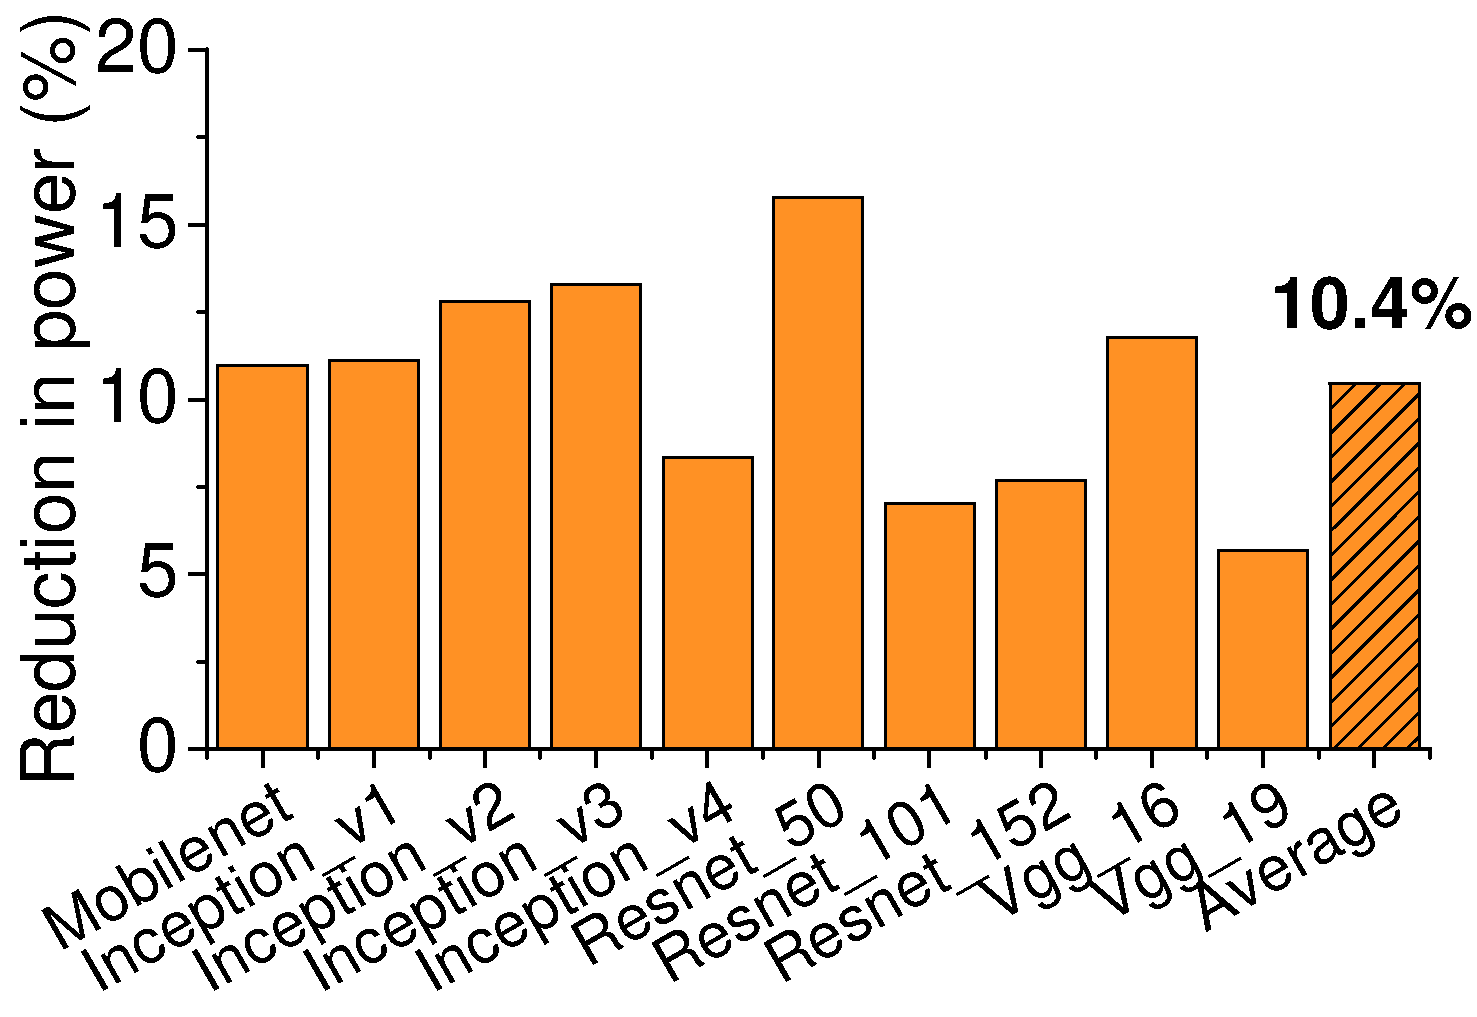
\includegraphics[width=0.3\textwidth]{figure/quan_power.pdf}}
\hfill
\subfloat[][Energy consumption]{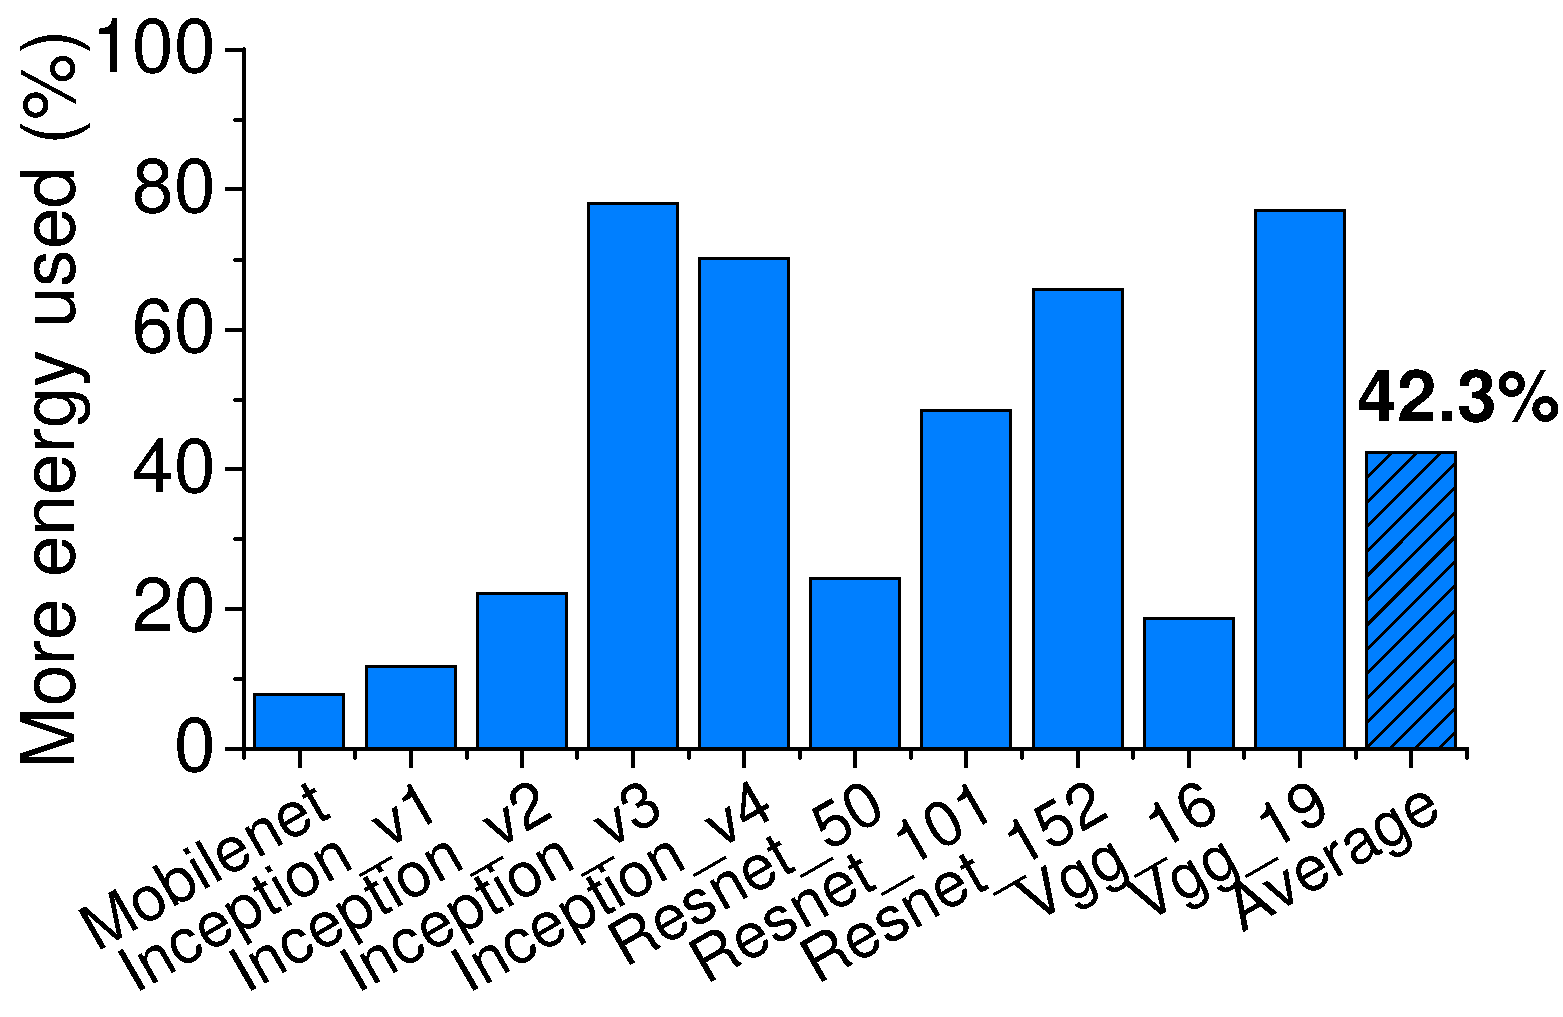
\includegraphics[width=0.3\textwidth]{figure/quan_energy.pdf}}
\hfill
\subfloat[][precision, recall and F1 score]{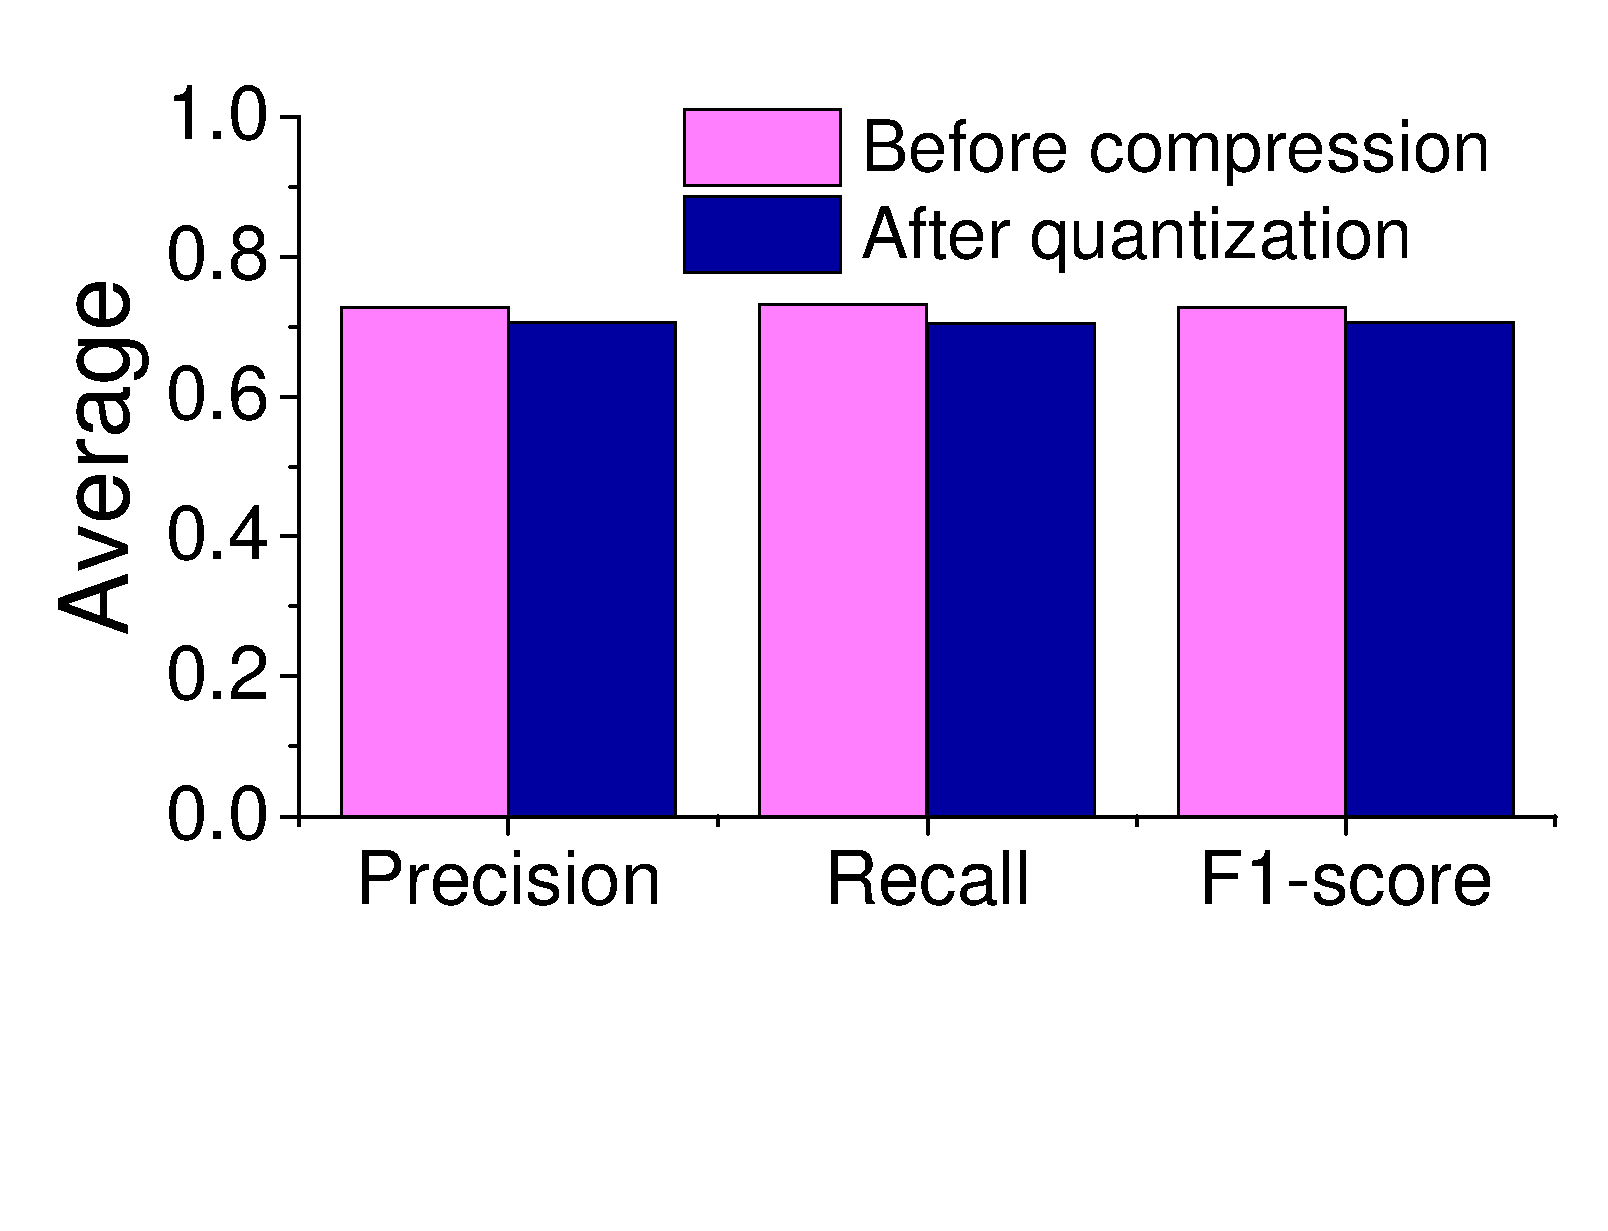
\includegraphics[width=0.28\textwidth]{figure/quan_prf.pdf}}
\hfill

\caption{The achieved model size (a) inference time (b) accuracy (c) power consumption (d)
energy consumption (e) and precision, recall and F1 score (e) before and after the compression by \quantization.
The compression technique to use depends on the optimization target.}
\label{fig:analy_quan}
\end{figure*}


\begin{figure*}[!t]
\centering
\subfloat[][Model size]{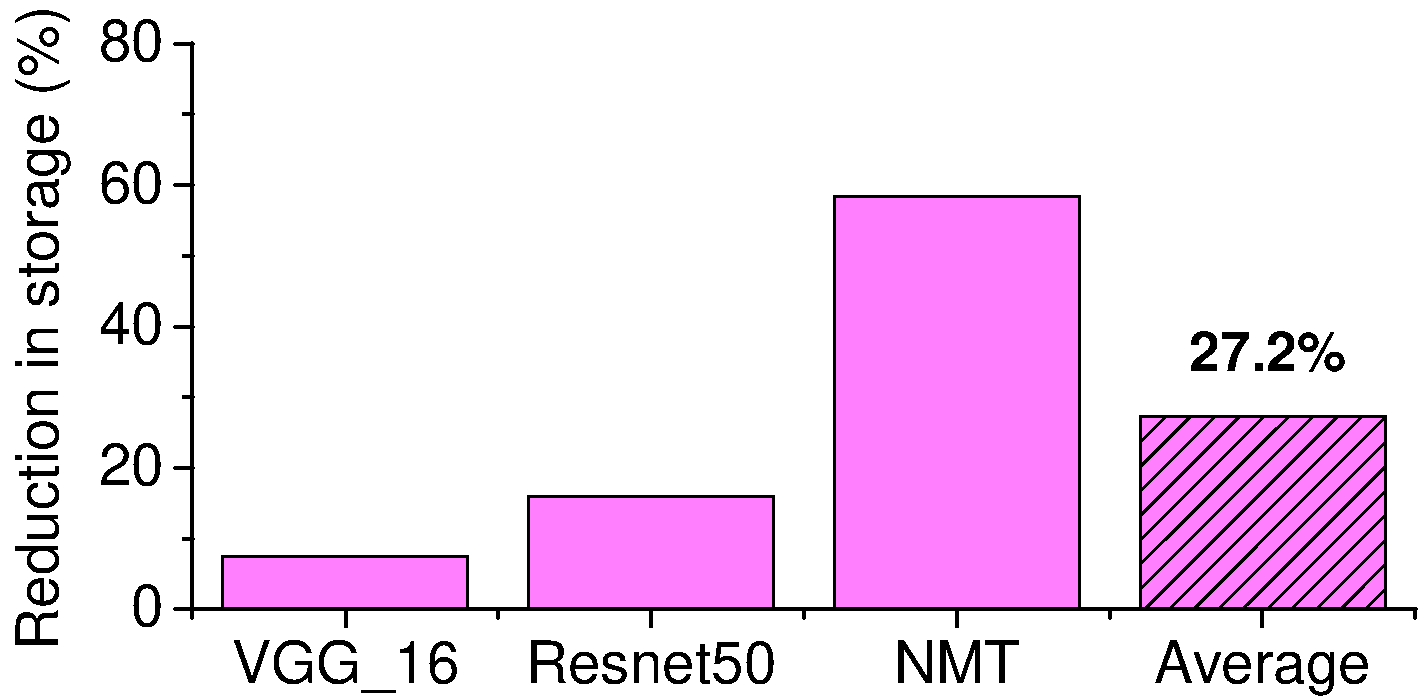
\includegraphics[width=0.33\textwidth]{figure/prun_size.pdf}}
\hfill
\subfloat[][Inference time]{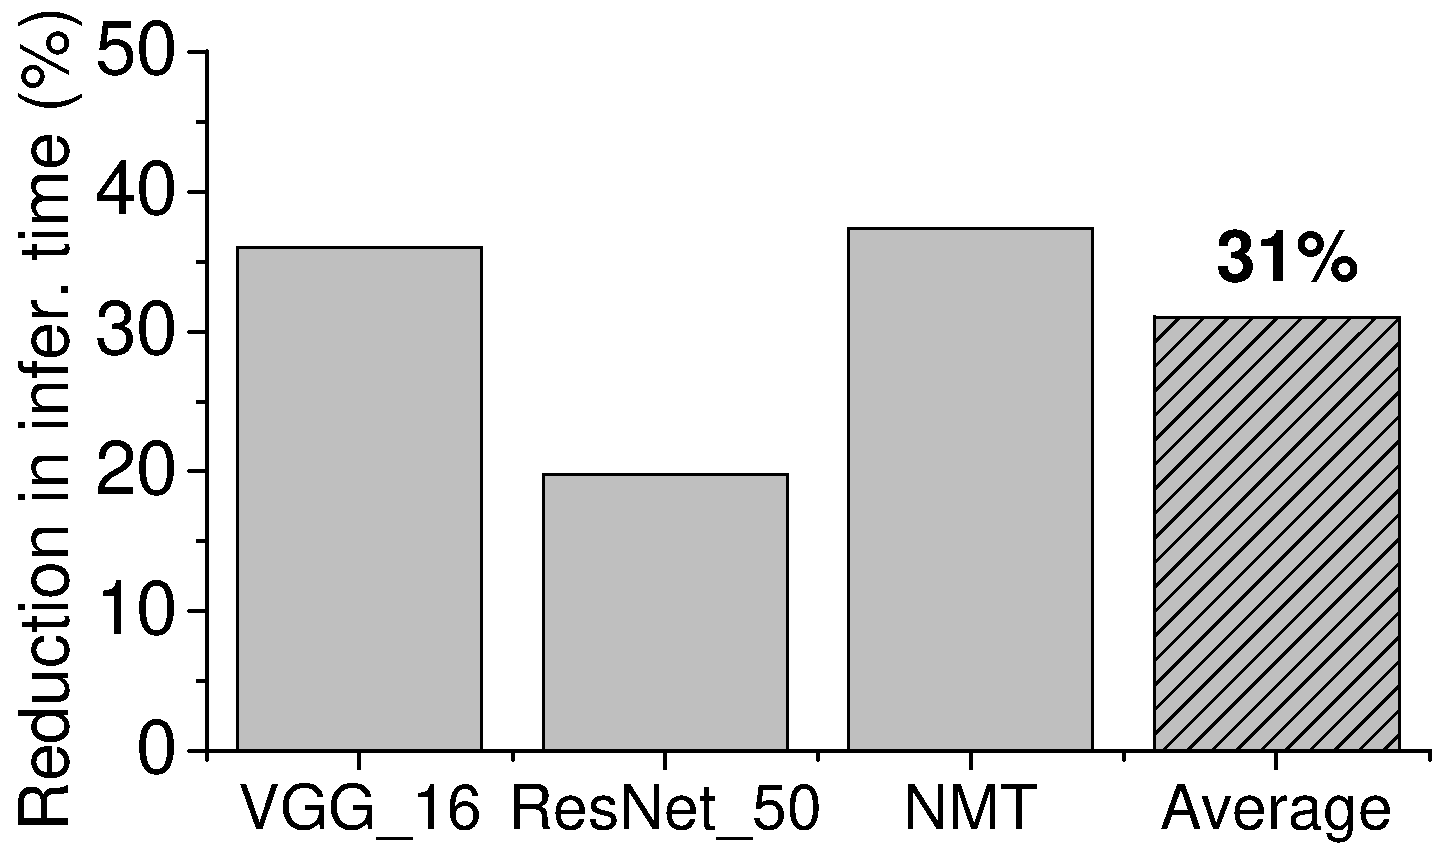
\includegraphics[width=0.3\textwidth]{figure/prun_time.pdf}}
\hfill
\subfloat[][Accuracy]{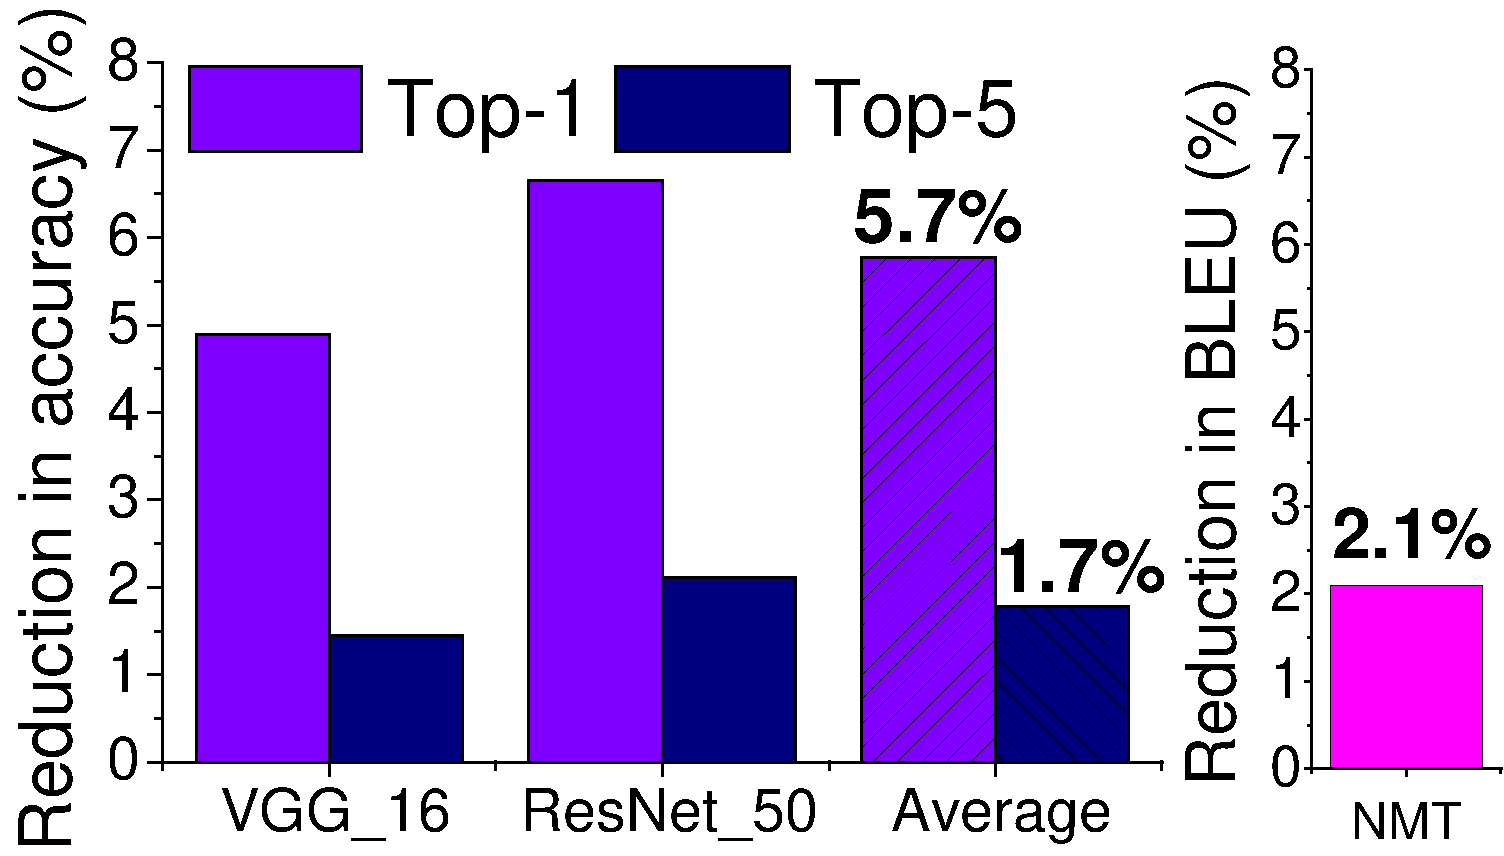
\includegraphics[width=0.3\textwidth]{figure/top1_5_prun.pdf}}
\hfill
\subfloat[][Power consumption]{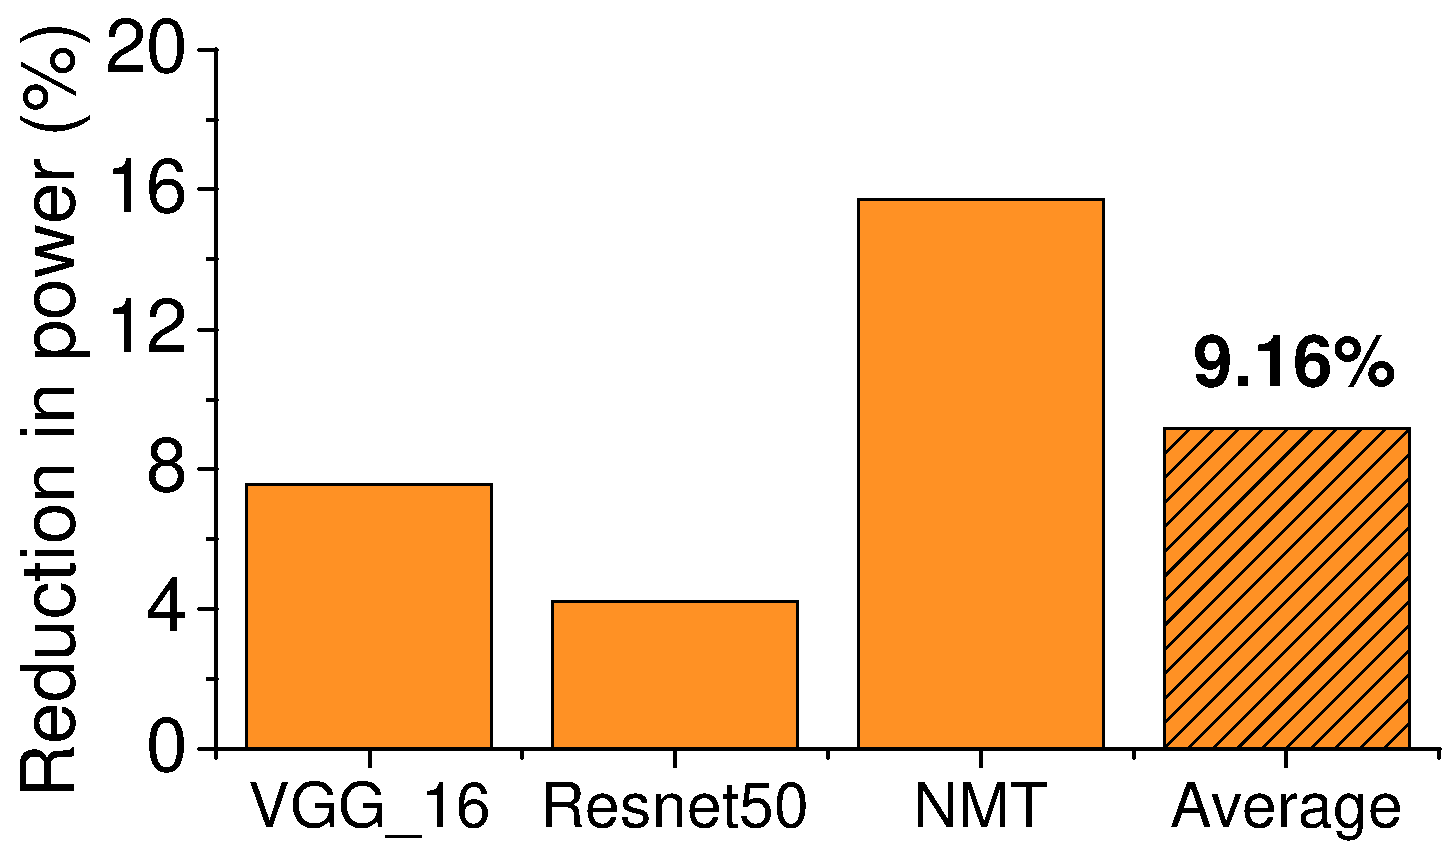
\includegraphics[width=0.3\textwidth]{figure/prun_power.pdf}}
\hfill
\subfloat[][Energy consumption]{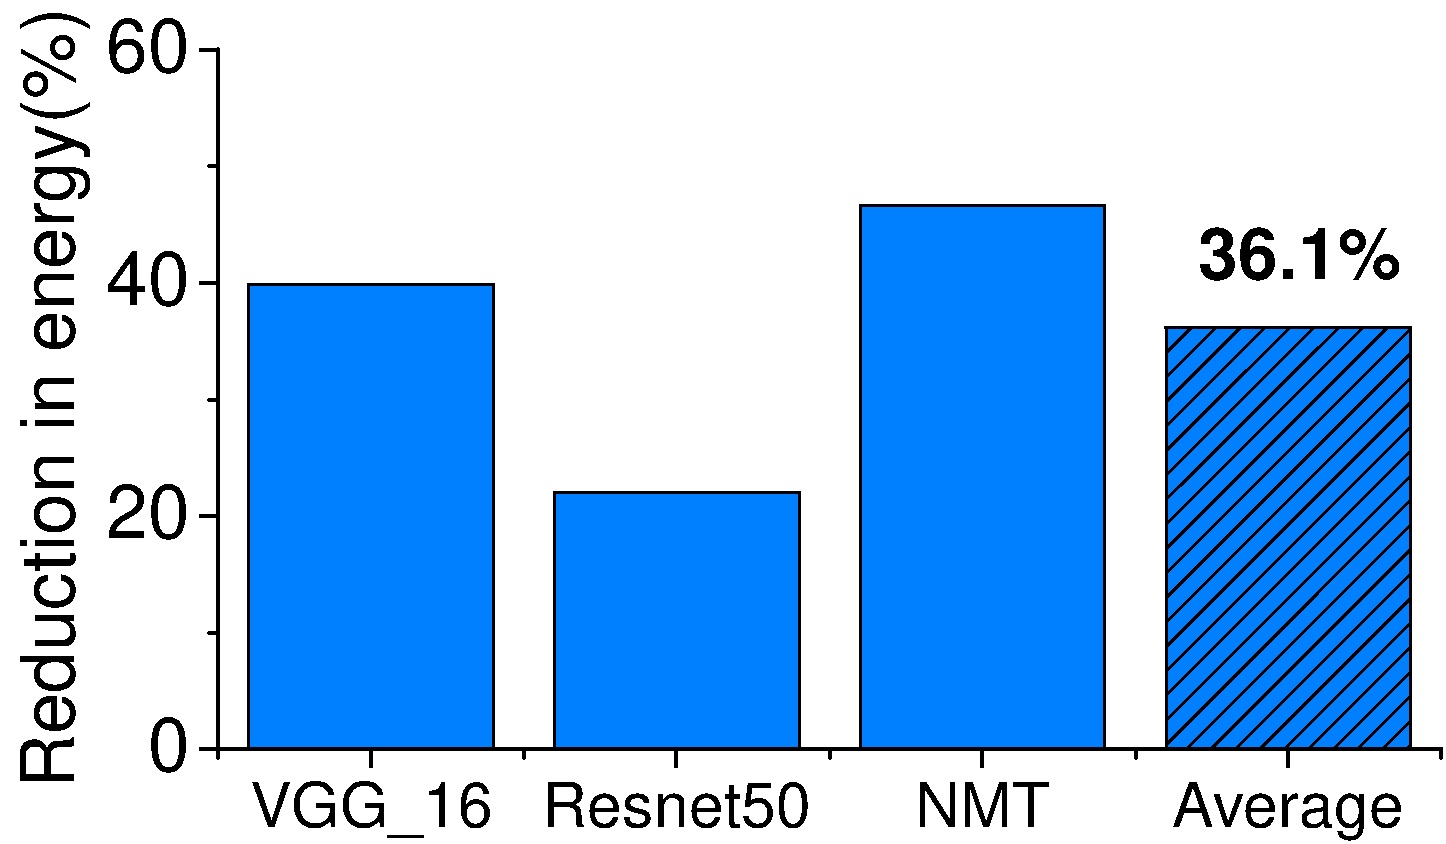
\includegraphics[width=0.3\textwidth]{figure/prun_energy.pdf}}
\hfill
\subfloat[][precision, recall and F1 score]{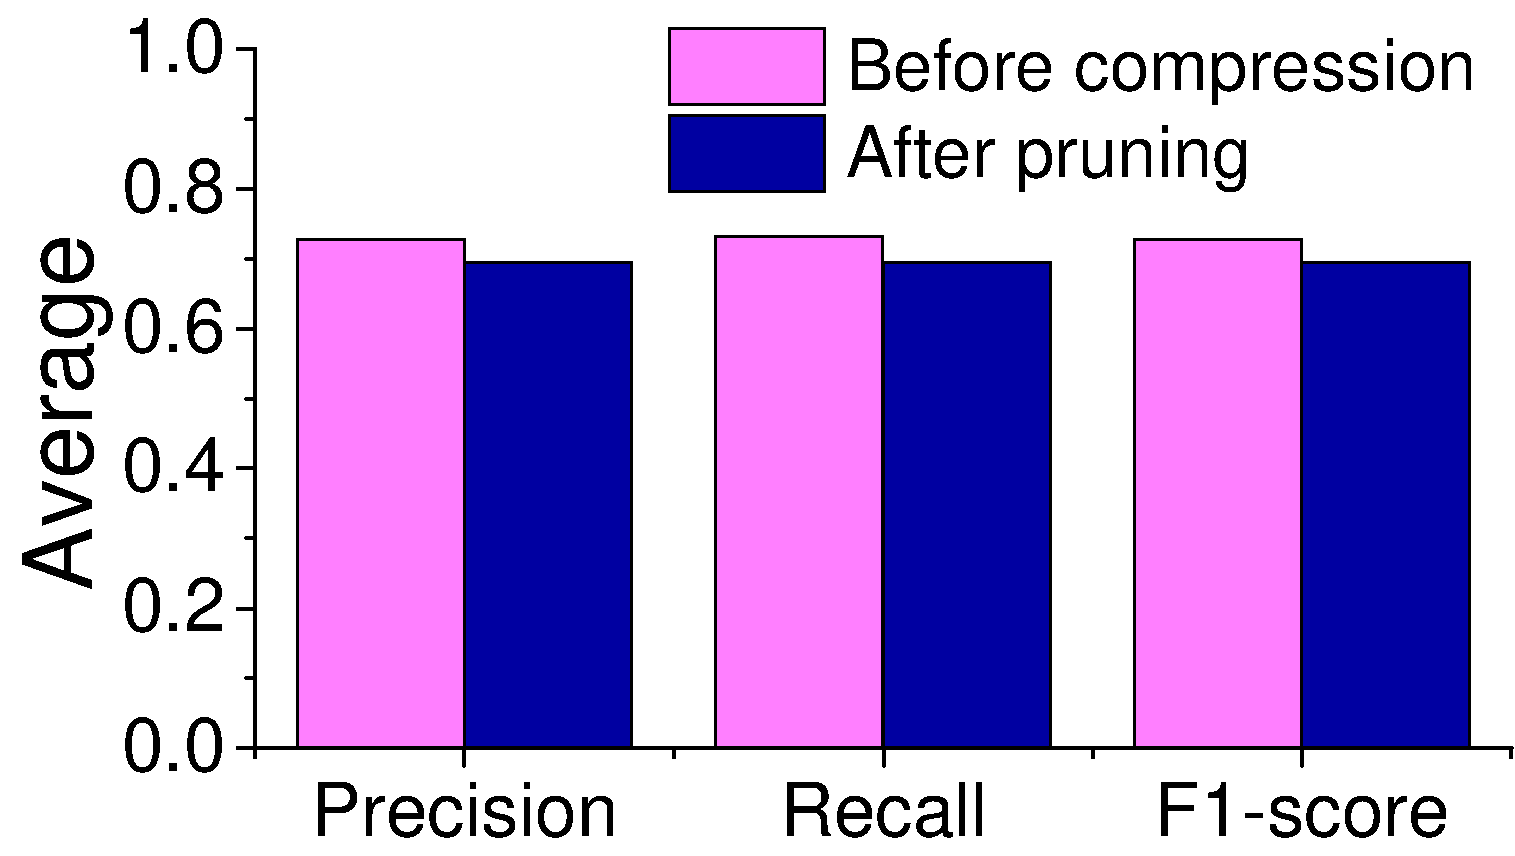
\includegraphics[width=0.3\textwidth]{figure/prun_prf.pdf}}
\hfill

\caption{The change of the model size (a), inference time (b), accuracy/BLEU (c), power (d), energy consumption (e), and accuracy (e)
before and after applying \pruning.} \label{fig:analy_prun}
\end{figure*}

\section{Experimental Results}


\subsection{Roadmap}
Our experiments try to answer the following questions:

\begin{itemize}
\item bla
\item bla2
\item bla3
\end{itemize}

\subsection{Impact on the Model Storage Size}
Reducing the model storage size is crucial for embedded and IoT systems which often have a limited storage space. A smaller model size also
translates to smaller runtime memory footprint of less RAM space consumption. Figures~\ref{fig:analy_quan} and  \ref{fig:analy_prun}
illustrate how the different compression techniques and parameters affect the resulting model size.

As can be seen from Figure~\ref{fig:analy_quan} a, using an 8-bit data quantization can significantly reduce the model storage size,
leading to an average reduction of 74.5\%. From Figure~\ref{fig:analy_prun} a, we see that by removing some of the pathways of the neural
network, \pruning can also reduce the model size, although the gain is smaller than \quantization. On average, \pruning reduces the model
size by 27.2\% (\FIXME{xx MB}). An interesting observation is that, \pruning is particularly effective for obtaining a compact model for
NMT, an \RNN, with a reduction of 60\% on the model size. This is because there are typically many repetitive pathways in an \RNN due to
the natural of the network architecture. As we will discuss later, \pruning only leads to a minor degradation in the prediction accuracy
for NMT. This suggests that \pruning can be an effective model compression technique for \RNNs.



\subsection{Impact on Accuracy Metrics}
When compressing a model, we still want to largely maintain the performance of a compressed model. Therefore, it is importance to
effectively trade precision for storage space. Results in Figure~\ref{} compare how the prediction accuracy metrics are affected by model
compression.

We see that the sweat spot of \quantization depends on the neural network structure. Although an 8-bit representation leads to a minor
decrease in the prediction accuracy, a further reduction of a 6-bit representation is only profitable for xx networks.

\subsection{Impact on Inference Time}


\subsection{Impact on the Energy Consumption}


\subsection{Memory footprint}
\begin{figure}[!t]
\centering
\subfloat[][\quantization]{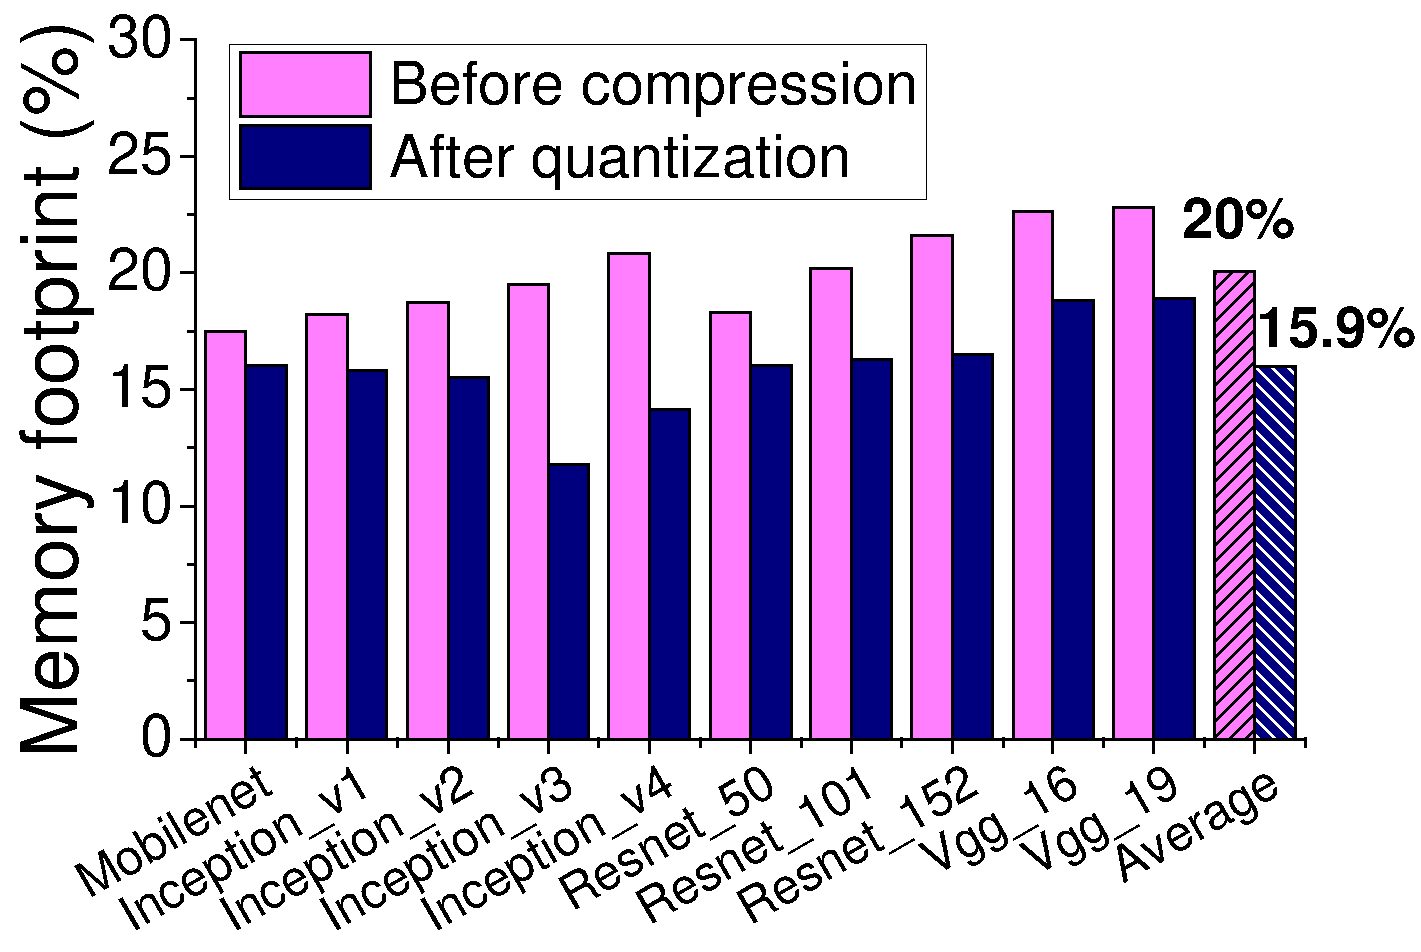
\includegraphics[width=0.23\textwidth]{figure/quan_mem.pdf}}
\hfill
\subfloat[][\pruning]{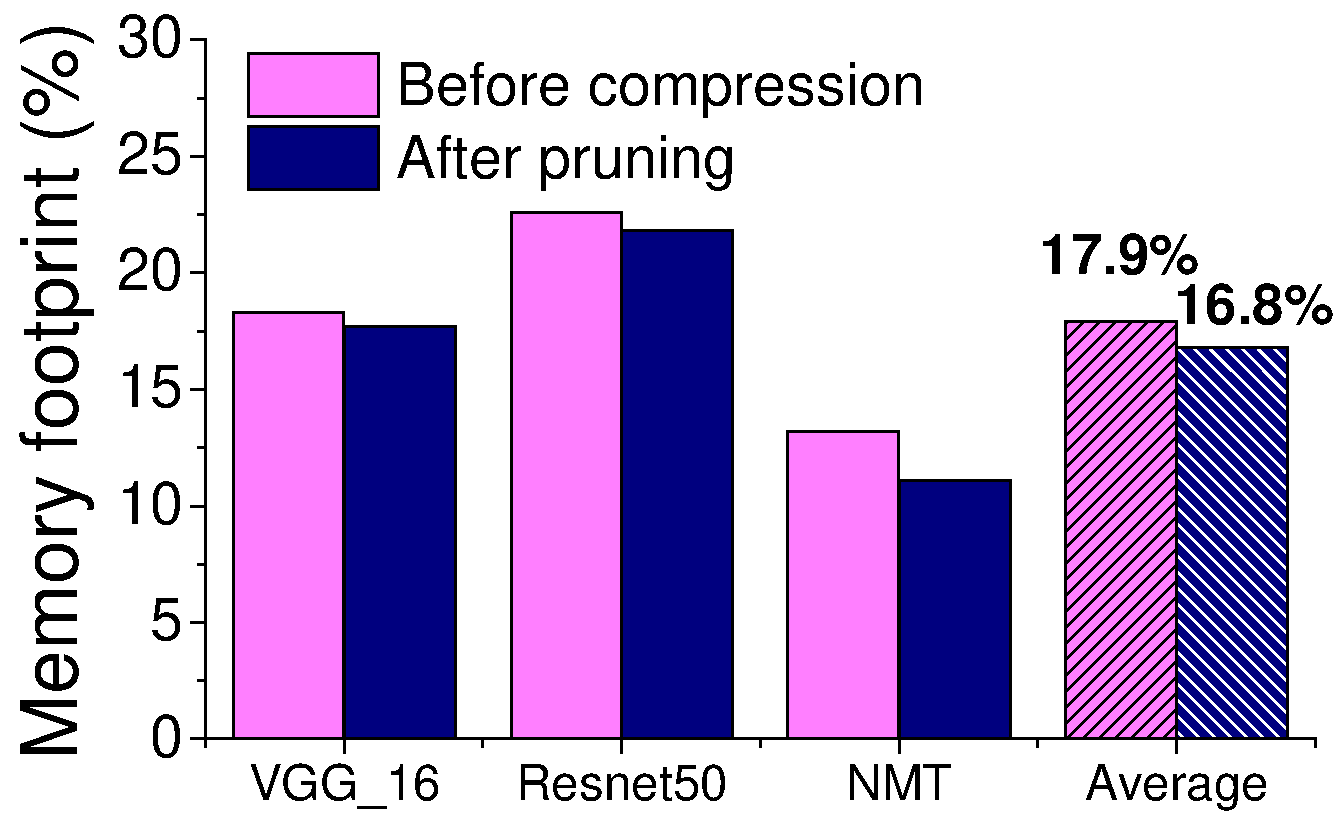
\includegraphics[width=0.23\textwidth]{figure/prun_mem.pdf}}
\hfill

\caption{Memory footprint before and after the compression by \quantization(a) and \pruning (b).}
\label{fig:footprint}
\end{figure}
